\documentclass[a4paper,12pt]{article}
\usepackage[english]{babel}
\usepackage[utf8]{inputenc}

\usepackage[top=2.5cm, bottom=2.5cm, left=2cm, right=2cm]{geometry}

\usepackage{datetime}
\newdateformat{monthyeardate}{%
  \monthname[\THEMONTH], \THEYEAR}

% Math packages
\usepackage{mathtools}
\usepackage{amsmath}
\usepackage{amsfonts}
\usepackage{amssymb}

\usepackage{enumitem}
\usepackage{algorithm}
\usepackage{algpseudocode}

\usepackage{listings}

\usepackage{makecell}

\usepackage[hidelinks]{hyperref}

\title{Mobile and Social Sensing Systems}
\author{Francesco Barbarulo, Giovan Battista Rolandi}
\date{\monthyeardate\today}

\begin{document}
\pagenumbering{roman}

\maketitle
\abstract{The aim of these notes is to give some pills of every argument for the oral test. We have assumed that the reader has attended the lessons because these notes, by themselves, are not sufficient to have a global and profound knowledge.

We wish you good luck!}

\tableofcontents

\newpage

\pagenumbering{arabic}

\section{Introduction}
\subsection{Mobility}
\begin{itemize}
  \item \textbf{physical}: hardware actually changes its physical position
  \item \textbf{logical}: applications and data may need to be moved for design reasons
\end{itemize}

\section{Localization systems}
Localization systems consist of two main blocks:
\begin{enumerate}[label=\roman*.]
	\item Set of deployed nodes with different \textit{states}:
		\begin{itemize}
		 	\item \textbf{beacon} (\textit{landmarks} or \textit{anchors}): already know their locations through a manual configuration or through GPS reading;
		  	\item \textbf{unknown} (\textit{targets}): do not have any information about their geographic locations;
		  	\item \textbf{settled}: targets nodes that has determined or estimated their locations.
		\end{itemize}
	\item Localization algorithm:
		\begin{itemize}
			\item GPS not longer used in CPS for cost and energy constraints;
			\item GPS-free techniques exploit the sensing and the wireless communication capabilities of CPS components
		\end{itemize}
\end{enumerate}

\subsection{Topology}
The topology of a localization algorithm refers to \textit{where} and \textit{how} the location of a given node is calculated:

\begin{itemize}
	\item \textbf{Centralized localizaiton}: a central device estimates the location of unknown nodes based on the signal measurements forwarded by anchors;
	\item \textbf{Localized localization}: each object estimates its location using the collected signal measurements and location information of the anchor nodes in its neighbourhood.
\end{itemize}

We can distinguish four different system topologies for localization systems, as shown in Figure~\ref{fig:topology}.
\begin{figure}[H]
	\centering
  	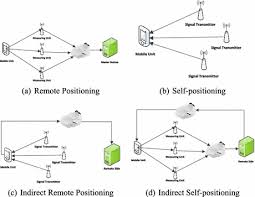
\includegraphics[width=0.4\textwidth]{img/topology}
  	\caption{\label{fig:topology}Taxonomy of localization systems topology}
\end{figure}

\subsection{Coordinate System}
Coordinates:
\begin{itemize}
  \item physical
  \item symbolic
  \item absolute
  \item relative
\end{itemize}

Communication paradigm:
\begin{itemize}
  \item non-cooperative
  \item cooperative
  \item opportunistic
\end{itemize}

Metrics:
\begin{itemize}
  \item accuracy: mean distance error
  \item precision: CDF of distance error
  \item complexity: hardware and/or software
  \item robustness: behavior under extreme conditions
  \item scalability: geographical and density
  \item cost
\end{itemize}



\end{document}